\documentclass{ltjsbook}
\usepackage{docmute} 
\usepackage{../../myStyle} 

\begin{document}
\setcounter{chapter}{7}
\chapter{システム論からみた社会心理学}
\label{sp08_system}

\section{はじめに}
前回までで，先週は学際休みだったんですけど，社会心理学\index[termidx]{しゃかいしんりがく@社会心理学}の現代に至るまでの歴史的なところはお話ししたつもりなんですが，今日からは話題が変わります。2つ目の話題に行こうと思っています。最初の授業の時にも一応3部作でという話はしてましたが，その2部目に今日から突入します。今日のお話はシステム論\index[termidx]{しすてむろん@システム論}というところです。

このシステム論\index[termidx]{しすてむろん@システム論}の話も多分2回，いや，2回は無理かな，3，4回はかかるかなと思っています。システムって，日本語で「系」という字を書くんですね。このシステム論\index[termidx]{しすてむろん@システム論}というのは，どこかの学部で，またはどこかの学科で体系的に教えられるということは，おそらくほとんどないんじゃないかなと思います。唯一，僕は昔看護学校で非常勤したことがあるんですが，そこにはシステム論\index[termidx]{しすてむろん@システム論}の授業がありました。その時もシステム論\index[termidx]{しすてむろん@システム論}というのは本当にシステム論\index[termidx]{しすてむろん@システム論}ですかと，それだけで単体の授業として成立するんですかと聞いたぐらい，ここだけ取り出して授業にしているところは少ないんじゃないかなと思います。

一体システム論\index[termidx]{しすてむろん@システム論}というのは何の話をするのかというと，科学の具体的な研究テーマやリサーチクエスチョンがある話というよりは，科学観，ものの見方に基づいて論じられるものです。システム論\index[termidx]{しすてむろん@システム論}としての共通した問題意識というのはあるんですけれども，それが何学なのかというのがわかりません。どこに分類して良いかがわからないというべきかな。

この授業は社会心理学\index[termidx]{しゃかいしんりがく@社会心理学}の授業ですが，社会心理学\index[termidx]{しゃかいしんりがく@社会心理学}の枠組みの中でシステム論\index[termidx]{しすてむろん@システム論}を中心に扱うことは多分少ないんじゃないかなと思います。

今日はこのシステム論\index[termidx]{しすてむろん@システム論}の歴史の話をします。システム論\index[termidx]{しすてむろん@システム論}の歴史というのは，スタートは生物学，その後化学の方で発展し，その次に神経科学の方で発展しました。その後コンピュータ科学，社会心理学\index[termidx]{しゃかいしんりがく@社会心理学}で発展した，と私は考えています。つまり，最終的には人文社会科学の枠組みでこれを話そうと思っています。ことほど左様に，学問領域を移動しながら学際的なものの見方に関するもので，見立ての学という側面があるものですから，ちょっと正体がつかみにくくて，教えた方もこれですよと，これがわかったらこういうことができるというのが伝えにくい形になっています。

歴史の話は社会心理学\index[termidx]{しゃかいしんりがく@社会心理学}の歴史を追いかけてきたから良かったんですが，今回はそういったものの見方になりますので，ますます抽象的な変な話になるかなと思います。なぜ冒頭にこのようなことを言うかというと，いきなりシステム論\index[termidx]{しすてむろん@システム論}を言い出して，しゃべり出してもいいんですが，ある程度のオリエンテーションがないと，受講生の皆さんも何を聞いてるんだろうとなるんじゃないかなと思ったからなんですね。

さて，これから何回かに分けてシステム論\index[termidx]{しすてむろん@システム論}のお話をしますが，確実にお約束できるのは，私は社会心理学\index[termidx]{しゃかいしんりがく@社会心理学}を考える上で，このシステム論\index[termidx]{しすてむろん@システム論}の考え方が必要だと思っているという点です。このシステム論\index[termidx]{しすてむろん@システム論}的な観点から社会心理学\index[termidx]{しゃかいしんりがく@社会心理学}を考えるということをしたい，皆さんにもしてもらいたいんです。なので，ちょっと変な，例えば生物学だとか化学の話をしているなと思ったとしても，そこの根底にあるのは社会心理学\index[termidx]{しゃかいしんりがく@社会心理学}を捉えるためのものの見方ということです。「システムとして社会心理学\index[termidx]{しゃかいしんりがく@社会心理学}を考える」という軸はブレずに行きたいと思っておりますので，よろしくお付き合いいただければと思います。

\section{システム論の背景}
さて，システム論\index[termidx]{しすてむろん@システム論}なんですが，これはどういった背景から出てきているかというと，単純に言って，「生きてるって何だろう」ということなんです。「生命」とは何か，ということを考えるための科学観，学問観としてスタートしています。生命とは何か，生きてるって何か，命とは何か，心とは何かというのは，非常に大きな問いです。しかし，これを考えるときに，「神様がくれたものだ」という考え方ではなく，科学的に考えるためにはどういった観点が必要なのか，というところからお話をしていきたいと思います。

この授業では以前，現代科学の基盤ということで，4つほど特徴を挙げさせていただきました。1つ目が実験的なアプローチです。ルネサンス前の時代に，ケプラー\index[nameidx]{けぷらー@ケプラー}やガリレオ\index[nameidx]{がりれお@ガリレオ}などは，聖書に書いてあることを全面的に信じるのではなく，ピサの斜塔から鉄球を落とすといった実験をすることによって，本当に書かれていることが確かなのか確認しようというアプローチをしたんですね。それまでは宗教的，キリスト中心的，教会中心的な考え方だったのですが，そこから自然科学的，実験的なアプローチが出てきたというのが，現代科学の一つの特徴だとお話しました。

第2の特徴は何かというと，1つは数学的還元主義，数値主義といった考え方です。ニュートン\index[nameidx]{にゅーとん@ニュートン}などに代表される考え方ですが，それが一体研究しようとしている対象，それが一体何なのかということではなく，それをどのようにして表現するか，どのように表すかという方法を数学的な関数で表現しましょうという考え方です。特に数学的に表現するという信念が，近代科学の一つのやり方です。数式というのは，文系の人はあまりそれを好みませんが，非常に厳密性の高い言語だといえます。だから，数学で表現するというのがサイエンスの知識の積み重ねには必要だったわけです。

それと，3つ目として，機械論的な発想というのを挙げておきました。デカルト\index[nameidx]{でかると@デカルト}が提案した格率，方法論の中に書いてあるんですが，彼は近代的な考え方を提案するんですね。デカルト\index[nameidx]{でかると@デカルト}が言いたい機械論的な発想というのは，こういう原因があったらこういう結果にたどり着きますよね，こういうメカニズムで，この順番で物事が動きますねという因果的なプロセスを考えるという発想です。

何だかわからないけど，急に突然何かが現れるんだというのではなくて，おそらく原因があるはずだ，ということです。現象には原因があるだろう，結果を生む何らかのメカニズムがあるだろうと。マクスウェル\index[nameidx]{まくすうぇる@マクスウェル}のデーモン，という譬え話がありますが，マクスウェル\index[nameidx]{まくすうぇる@マクスウェル}\footnote{ジェームズ・クラーク・マクスウェル\index[nameidx]{まくすうぇる@マクスウェル}(James Clerk Maxwell，1831年6月13日 - 1879年11月5日)は，マクスウェル\index[nameidx]{まくすうぇる@マクスウェル}の方程式を確立し，電磁気学や統計力学で重要な業績を残したスコットランドの理論物理学者です。(Wikipediaより)}が考えたのは，ある特定の時間の空間にある全ての分子，原子の位置と速度，運動が分かる悪魔がいたら，この先何が起こるかを完全に予測できるだろうという全知全能の存在です。実際にそういう悪魔がいるかどうかという話は抜きにして，大事なのはその発想です。すべての条件を確実に全部把握すれば，因果のつながりで未来までしっかりと寸分違わず予測できますよ。なぜなら，それは物が動くには不思議な神秘的な力がかかっているのではなく，メカニズムがあるからですよ，というわけですね。そういうメカニズムに基づく考え方，というのがこの機械論的な発想です。これが近代科学の特徴の三つ目。

そして四つ目は，これもデカルト\index[nameidx]{でかると@デカルト}の格率ですが，分解と統合です。大きな問題は小さなパートに分けて，それを組み立てていけば，最終的には全体を理解したことになる，という考え方ですね。これは要素還元主義とも言われます。小さな要素に還元して，大きな複雑な問題は小分けにして考えていきましょう，というスタイルですね。

ということで，今挙げました実験的なアプローチ，数値主義，数学的な現象主義，機械論的な発想，因果的な発想と要素還元主義，これが近代科学の発想，考え方の根本なんですけれども，このアプローチでもっても捉えられないのが，生命というものです。生きているとはどういうことか，ということを考えるときに，今言ったようなアプローチが効かないわけですね。このアプローチでは生命ということの解明ができないというのが大きな問題なわけです。

すぐにお分かりいただけるかと思うんですが，要素還元主義的に生命にアプローチしようとして，生きている人間をズバーッと切って，「さあどこが生きている要素なのかな」と言って，例えば上半身とか下半身に切り分けてみました。「どっちが生きているんだろう」と思ったら，両方死んでしまいました，みたいなことになりますよね。これは当たり前です。生きているっていうのは分けても分からないんです。では，何が原因でどういうメカニズムができているのか。もちろん体の中の色々な仕組みについては，どういう原因でどういう結果というような物理学，化学の法則に従って動くのでしょうけれども，そもそもどのようにして生命のようなものが作られているかというような問いには答えられないわけですね。誰しもが不思議に思う「生命がある」，「命がある」ということを，近代科学的なアプローチでは答えが出せないんです。考え方ではアプローチで答えが出せないので，おそらく抜本的な発想の転換が必要だろうというわけですね。

生きていることの不思議さの一つは，有機体が持っている，再生する，成長する，増殖するという特徴ですね。爪を切っても生えてきます，髪の毛を切っても生えてきます，そして新陳代謝によって私たちの体の細胞は3ヶ月もすれば全て入れ替わっているとか言われるんですけれども，その割には3ヶ月前の私と今の私は同じだ，と誰しも考えています。どうやってそんなことが成立しているのか。つまり私を構成する物質的な要素を全部分解して並べてみても，構成してもできないわけですね。その中心には何だか分からないが，生命というもの，何か一体のあるそれね，これが言葉にしにくいところなんですけど，ここでは生命ですから命とか生命ということを言っておきますが，生きている生き物というのは自身というのを常に生産している。何だったらずっと成長している。

今週の水曜日に私の娘が誕生日を迎えて14歳になったんですが，昔の写真とか見ていると，これが同じ物質とは思えないですよ，ほんとに。当然同じ物質，物理的には同じものではないんですよね。サイズが違いますからね。
ただ，本人はこの頃の写真の記憶があるとかって言ったりするわけです。どのようにして変わりながら同じであり続けるものを我々は維持しているのか，そしてそれを少しも不思議と思わないわけですよね。だからこの辺がもう真面目に考えると不思議で仕方がないわけです。

「増殖」と書いてあるのは，もちろん細胞分裂的な自己が増殖するということもありますし，自分の情報を持ったよく似た同じようなものを作ることができる，というのもそれかもしれませんね。今言いましたように僕には子供がいますから，分身を作れてるわけです。生命というのは紡がれますから。これは近代科学の実験的にやってみようとか，分解してみようとか，何かが原因で，また親が原因で子供が生まれるみたいな雑な話だったらそれでもいいんですけど，原因と結果の，しかもその分かりやすいものでもない，数学的に厳密に表現できるものでもない，これをどう捉えたらいいのかというのが難しいわけですね。

確か数年前に，講談社現代新書で，「生命は分けても分からない」という本がベストセラーになりました\parencite{FukuokaShin1}。
10年ぐらい前だったかな。それぐらいになるかもしれませんけど，福岡伸一\index[nameidx]{ふくおかしんいち@福岡伸一}さんという方が書いておられる本です。軽い読み物なので読んでみてください。そこには，ハッキリとタイトルにある通り，分けても分かりません，分解しても分かりませんというようなことが書いてあります。要素還元主義的に生命というのは研究できませんよというのは，もう誰しもが分かっているところなわけですね。くどいようですが，生きているものを分解すると，その時点で生きているものではなくなる，死んでしまうということがあるわけです。しかも，これも不思議なことに，我々生き物というのは，相手が生きているか生きていないかというのは，結構すぐに判別できるという能力も持っていますね。何か相手が意志を持ってそうだ，心を持ってそうだ，命を持ってそうだというようなことは，我々は比較的早々に判別できるんですけれども，そういった特徴がある生命というものを考えないわけにはいかんだろうというわけです。

生命の世界は，因果的でもないです。近代科学でいうところの因果の考え方というのは，AだったらB，Aが原因で原因があるから結果があるという，一方向な感じの考え方ですね。しかし，人間がすること，生命がすること，あるいはそういったものが織りなすものというのは，何が原因で何が結果になっているのかがわからない。この一つの原因が，一つの結果を及ぼすというのが，因果関係を特定するためにというような基本的なアイデアです。

因果関係というのはどうやって特定するかというと，まず原因と結果というのが確実にあって，しかも原因の方が時間的に先行している必要があります。当たり前ですね。結果が先に来て，結果があったから原因が生まれたということであれば，言葉の語義矛盾ですから。時間的に原因の方が先にあって，結果の方が後にあるという必要があります。ほかにも因果関係を特定するためには，AがBになりますよというときは，Aという原因がB'にはなりませんし，CにもDにもなりませんよ，ということが言えないといけない。AがBだけになりますという，すごく方向的な1対1の関係を言うわけですね。もちろんのことながら，他の要素が結果に結びつくというのもダメです。EもBの原因ですよ，FもBの原因ですよ，どれかが原因ですよというようなのは，因果関係を特定したとは言いません。因果関係というのは「原因が確実にこの結果を引き起こします」，という説明スタイルになっているわけです。この一方向的で時間の順序があって，一意性があるということが必要です。

それらが満たされた上で，「AならばB」という考え方を持ってきます。ここが，理論的に因果関係をつなげる発想です。しかし，ヒューム\index[nameidx]{ひゅーむ@ヒューム}が言ったように\footnote{ヒューム\index[nameidx]{ひゅーむ@ヒューム}の呪い(Hume's Curse)は，哲学者デイヴィッド・ヒューム\index[nameidx]{ひゅーむ@ヒューム}が提唱した因果性への懐疑や「事実(is)」から「価値(ought)」を導けないという議論を指します。この概念は，因果関係を安易に信じることへの警告や，倫理的判断の困難さを表現する際に用いられます。(Wikipediaより)}，「昨日も今日も朝太陽が昇ったからと言って，明日も太陽が昇る保障がどこにあるのか」といわれたら，もう困っちゃいますね。朝になれば太陽が昇るというのは，たしかに今までずっとそうだったけど，明日がそうである保障は別にないわけです。これが原因だからこれが結果，という順番で因果関係が起こるというのは，あくまで見ている人の見立てに過ぎないという考え方も，もちろんあり得るわけです。

さて，それから考えると，近代科学はわざと因果を一方向，すごく限定的な意味で使うことによって成立しています。しかし，生命や，生命をはじめとする生き生きしているもの，これらを表現するときには，近代科学的な発想というのは，いろいろとそぐわないわけですね。生命というのは，自分も生きていますし，皆さんも生きています。ものすごく身近にある話なんですけれども，その神秘性は，近代科学的なアプローチではわからないということです。これを何とか理解しようというのが，今日お話しするシステム論\index[termidx]{しすてむろん@システム論}です。

そういった意味で，生命を考えるというところからシステム論\index[termidx]{しすてむろん@システム論}というのは始まっています。システム論\index[termidx]{しすてむろん@システム論}という生命を考えるためのディスカッションは，いろんなところに応用できます。生きているのは必ずしも，1個人，1つの生命だけを対象にした学問ではなくて，「システム」という単位で考えましょうという考え方です。

\section{システムで考えよう}
「システム」とは，何らかのひとまとまりという意味ですが，この用語は，皆さんもよく耳にしますよね。僕も子供の頃から「システム」という単語は聞いていると思います。システムという用語がついているものをいろいろ考えてみようということで，いくつか例を挙げてみます。社会システム，情報システム，制御システムなどの仕組み的な用語がありますね。また，教育システム，経済システム，政治システムなどを言ったりすることもあります。

心理学においては，人間のシステム，行動システム，家族システムなんていう考え方もあります。一般的な社会でも生産システムや人間システムという言い方をしますし，生き物を中心に考えたら，神経システム，免疫システムなんていうのがあります。系という言葉を使って表現すれば，循環器系や生態系というのもシステムですね。太陽系というのも英語ではソーラーシステムですし。

システムという言葉が最も身近なのは，おそらくコンピュータサイエンスのところです。オペレーティングシステム(OS)という言葉がありますよね。ほかにもデータベースシステム，ネットワークシステム，セキュリティシステム，通信システム・・・といった言葉の中に入っているこの「システム」という言葉の使い方から分かることは，生命や生体的な性質が垣間見えますし，何かのひとまとまりである，ということでしょうね。ここで定義しておくなら，「相互に影響し合う要素からなる全体」というのがシステムの言葉の定義です。相互に影響し合う要素からなる全体。皆さん，この言葉聞いたことあるような気がしませんか？要素からなる全体のこと。

しかも，システム論\index[termidx]{しすてむろん@システム論}を考えるときに言われるのは，生命は分けても分からないわけですから，全体は要素の総和以上である，ともいわれます。なんとかからなる全体を表現したいんですけど，この全体は要素の総和以上であるという特徴を持っている。要素に分けても分からないので，要素を超えた全体ですよ。その全体的なまとまりをシステムと呼んで，そのシステムについての学をやりましょうというのがシステム論\index[termidx]{しすてむろん@システム論}です。この要素が何でも良いというところも一つのポイントなので，押さえておいてください。

例えば情報システムでは，インプットがあり，メモリーがあり，プロセスによる演算処理があり，データの保存・読み出しをしながらビットを置き換えて出力するといった，一連の要素からなる処理体系があります。
あるいは会計システムを例に取ると，必要な品目などを人が入力すると，予算枠の中で適切に分類され，様々な要素で計算して，支払いや手続きを進めるといった流れがあります。このように，多くの要素が組み合わさった全体像のことを「会計システム」と呼んでいるわけです。

システム論\index[termidx]{しすてむろん@システム論}で重要なのは，個々の要素に分解することではなく，全体として捉えることです。これから学ぶシステム論\index[termidx]{しすてむろん@システム論}は，まさにこの考え方に基づいています。
そして，私が社会心理学\index[termidx]{しゃかいしんりがく@社会心理学}の文脈でシステム論\index[termidx]{しすてむろん@システム論}を扱おうとしているのは，集団や社会もまたシステムだからです。クルト・レヴィン\index[nameidx]{くると・れゔぃん@クルト・レヴィン}が指摘したように，グループとは，メンバーが相互に依存し合う，ダイナミックな全体性を持つものです。つまり，グループは生命体のような動きをする存在なのです。レヴィンもゲシュタルト心理学\index[termidx]{げしゅたるとしんりがく@ゲシュタルト心理学}も指摘しているように，全体は単なる要素の総和以上のものなのです。グループというのは，メンバーが相互に依存し合っていることが必要で，相互に依存し合うメンバーの総体，ダイナミックな全体性のことをグループと定義したわけですね。つまり，グループというのは，生命，生きたかのような動き方をする何かなんです。しかもレヴィンも，あるいはゲシュタルト心理学\index[termidx]{げしゅたるとしんりがく@ゲシュタルト心理学}のテーマでもありますが，全体は要素の総和以上ともいってる。ここのところをうまく心理学，社会心理学\index[termidx]{しゃかいしんりがく@社会心理学}の中に取り込みたいですね。

そのためには，社会心理学\index[termidx]{しゃかいしんりがく@社会心理学}の文脈はちょっとずれますけれども，生命を考えるというシステム論\index[termidx]{しすてむろん@システム論}の発想と結びつけることが重要です。これについて考えてみようという話をしていきたいわけです。

\section{システム論の系譜}
この話をするにあたって，いくつか本のご案内があるんですが，話のスタートはこれです。フォン・ベルタランフィ\index[nameidx]{べるたらんふぃ@ベルタランフィ}\footnote{ルートヴィヒ・フォン・ベルタランフィ\index[nameidx]{べるたらんふぃ@ベルタランフィ}(Ludwig von Bertalanffy，1901年9月19日 - 1972年6月12日)は，オーストリア出身の生物学者で，「一般システム理論」を提唱し，生命現象に対する機械論を排してシステム思考の基礎を築きました。彼の名は，魚類の成長を表す「ベルタランフィ\index[nameidx]{べるたらんふぃ@ベルタランフィ}の成長関数(VBGF)」にも残されています。(Wikipediaより)}という人が書いている「一般システム論\index[termidx]{しすてむろん@システム論}」というのがあります\parencite{vonBertalanffy}。これがシステムという言葉が全面に出てきた最初なので，興味がある人は読んでみてください。

この一般システム論\index[termidx]{しすてむろん@システム論}は学際的な理論です。生命現象を出発点としていますが，経済，政治，軍事，社会など，様々な分野にシステムの考え方を適用できます。「一般」(general)という言葉が示すように，これは広く応用可能な理論と位置付けられています。システム論\index[termidx]{しすてむろん@システム論}は本質的には物の見方の提供です。生命をシステムとして捉えたり，集団をシステムとして分析したりするような，ものの見方を示す理論です。この考え方，特に生命現象に関連する捉え方は，時代とともに徐々に変化してきました。

さて，ここにもう一冊別の本があるんですが，河本英夫\index[nameidx]{かわもとひでお@河本英夫}という人が書いているオートポイエシスという本があります\parencite{KawamotoHideo}。この本は1995年に出ています。この本の中には，今言ったシステム論\index[termidx]{しすてむろん@システム論}の歴史的な変遷がまとめられています。オートポイエシス(Autopiesis)という言葉は聞き慣れないと思いますが，これもお話しするつもりです。この本の中で書いてあるシステム論\index[termidx]{しすてむろん@システム論}の歴史的な変遷についてちょっと説明しておきますと，最初，第一世代システム\index[termidx]{だいいちせだいしすてむ@第一世代システム}というのが，今言いました一般システム理論から始まったものです。

\begin{table}[h!]
    \centering
    \caption{世代ごとのシステム論\index[termidx]{しすてむろん@システム論}の概要}
    \begin{tabular}{cccc}
    \hline
    世代 & テーマ & Theme in English & 背景領域  \\ \hline
    第一世代 & 動的平衡系\index[termidx]{どうてきへいこうけい@動的平衡系} & Dynamic Equilibrium & 生物学  \\ 
    第二世代 & 動的非平衡系\index[termidx]{どうてきひへいこうけい@動的非平衡系} & Dynamical Nonequilibrium Systems & 化学  \\ 
    第三世代 & 自己創出系 & Autopoiesis & 神経生理学 \\ 
    第四世代 & 複雑系\index[termidx]{ふくざつけい@複雑系} & Complex Systems & コンピュータ科学  \\ 
    第五世代 & ネットワーク系 & Complex Network Systems & 社会心理学\index[termidx]{しゃかいしんりがく@社会心理学} \\ \hline
    \end{tabular}
    \label{tab:system_generations}
\end{table}


理論としてはこうなんですけれども，どういったテーマを扱っているかというと，動的平衡系\index[termidx]{どうてきへいこうけい@動的平衡系}Dynamic Equilibriumといわれたりします。第二世代になりますと，どういうことをテーマにするかというと，これが面白いのですが，動的非平衡系\index[termidx]{どうてきひへいこうけい@動的非平衡系}になるんですね。第一世代システム\index[termidx]{だいいちせだいしすてむ@第一世代システム}で平衡って言ったんじゃないのかと思うかもしれませんが，第二世代システムは同的非平衡系です。あるいは別名，自己組織化系\index[termidx]{じこそしきかけい@自己組織化系}Self-Organization Systemというふうに呼ばれることもあります。そして，第三世代システムというのがオートポイエシスAutopoiesisなんです。名前が難しいと思うと思うので，これはまた順を追って説明しますが，これは自己創出系というテーマになります。このまとめ方は，河本の書いているオートポイエシスという本\parencite{KawamotoHideo}の中で表された考え方で，時代とともにこうやって考え方，テーマが変成してきましたよという話になっています。

ちなみに，10年くらい前に福岡先生の本，「生命は分けても分からない」\parencite{FukuokaShin1}が流行ったと言いましたが，あの先生が言っていらっしゃるのは動的平衡系\index[termidx]{どうてきへいこうけい@動的平衡系}です。生き物ってのは動的平衡系\index[termidx]{どうてきへいこうけい@動的平衡系}だよという話なんです。僕は最初に読んだときに，今更ですか?と思いました。まだ第一世代システム\index[termidx]{だいいちせだいしすてむ@第一世代システム}のことを言っているんですか?とね。いや，別に時代が後に来ているのが偉いとか偉くないとかっていうことは言いたいわけではないんですけど，理論というか考え方自体は進んでいっておりますので，そういったどういう変遷はあるかとか，どこに着目するか，どう変わっていったかというような視点で見ていただくとよろしいかなと思います。

さて，河本はこうやってですね，システム論\index[termidx]{しすてむろん@システム論}の進行を時系列的に1，2，3と分けました。さっきも言いましたが，これが1995年の話です。その後，僕が大学院生になろうとしていた頃ですから，95〜98年くらいの時は言われてませんでしたが，第4世代システムの議論が出てきています。それが複雑系\index[termidx]{ふくざつけい@複雑系}です。Complex Systemsですね。皆さん，この名前は聞いたことありますでしょうか?本当に2000年の頭の頃は，複雑系\index[termidx]{ふくざつけい@複雑系}というタイトルの本がいっぱいあちこちにあったんです。個人的にはミシェル・ワルドロップの書いている「複雑系\index[termidx]{ふくざつけい@複雑系}」\parencite{Waldrop}という本がストーリー仕立てで分かりやすいかなと思いますが，それに限らず，新書からハードカバーまで，いろんなものが複雑系\index[termidx]{ふくざつけい@複雑系}という話を扱ってました。この複雑系\index[termidx]{ふくざつけい@複雑系}というのは，コンピュータサイエンスなども相性がいいんですけれども，いわんとしていることは，まさに生命の捉え方です。複雑系\index[termidx]{ふくざつけい@複雑系}のテーマは，「複雑なものは複雑なまま」。単純化して考えようとするのがダメということですね。加えて複雑系\index[termidx]{ふくざつけい@複雑系}という観点は，要素同士の動きは単純であったとしても，複雑な要素が創発(emergence)されるという考え方で，表面だって見えている複雑さというのも，直接的に相互作用し合う要素同士からなる全体なんだという観点の話です。

これも，おいおいお話していきます。今日は，多分，第一世代システム\index[termidx]{だいいちせだいしすてむ@第一世代システム}の話ができませんが。

さて，4番目と5番目についてはまとめている人はいませんので，私なりの考え方なんですけれども，複合システム，あるいはネットワークシステムが第5世代かなと思います。ネットワークシステムというのは，基本的に要素が結びついて，ネットがワークするわけですから，結節点がつなぎ合って連動するというネットワークのシステム，その全体ということを考えましょうということなので，ネットワークシステムという話をしています。これをシステム論\index[termidx]{しすてむろん@システム論}の視点でしゃべったのが，私の学部の時の師匠である藤澤等\index[nameidx]{ふじさわひとし@藤澤等}です。

ちなみに，藤澤等\index[nameidx]{ふじさわひとし@藤澤等}の師匠である廣田君美というのが，一般システム論\index[termidx]{しすてむろん@システム論}の考え方でグループダイナミックス\index[termidx]{ぐるーぷだいなみっくす@グループダイナミックス}集団心理学をやろうとした方ですね。そういう意味で，僕はずっとシステム論\index[termidx]{しすてむろん@システム論}的な観点から社会心理学\index[termidx]{しゃかいしんりがく@社会心理学}を考えるというのを教わってきてる人間です。今からシステム論\index[termidx]{しすてむろん@システム論}の話をしていきますが，今後の流れとして，だいたいこういう感じで発展していくんだというのを先に見通しを立てておいていただければなと思います。

この授業では，上から順番に解説していくつもりですが，興味がある方は，例えば河本のオートポイエシスの本\parencite{KawamotoHideo}を読むとかすると，ポンと先読めたりするからいいかもしれません。ちなみに，複合システムネットワークについては，藤澤等\index[nameidx]{ふじさわひとし@藤澤等}が「複合システムネットワーク論」\parencite{fujisawaNetwork}という本を書いています。そこでは彼なりの別の観点からのシステム論\index[termidx]{しすてむろん@システム論}の分類というのをやっていて，多少その辺も面白いので興味があったら読んでみてください。

ちょっと余談になりますが，第一世代システム\index[termidx]{だいいちせだいしすてむ@第一世代システム}のスタートは生物学です。第2世代システムの中心というか，考え方のポイントは，生物学，化学というところからこの考え方が出てきています。さっきも言いましたが，オートポイエシスは神経生理学の方から来た話です。こちらはコンピュータ科学です。さらに，この複合システムネットワーク論は，個人的には社会心理学\index[termidx]{しゃかいしんりがく@社会心理学}からきたといいたいですが，ネットワークシステムという意味では，これもコンピュータ科学に入っていいかもしれません。それとも生命科学と言った方がいいのかな? 要は，人工知能，チャットGPTだとか，生成AI\index[termidx]{せいせいえーあい@生成AI}，大規模言語モデルだとか，それに基づく，それの元にある機械学習，ニューラルネットワークモデルみたいなものは，このネットワークを中心にしたサイエンスですから，こういった観点は持っているはずです。

ことほどいろんなところで語られているものだから，これが社会心理学\index[termidx]{しゃかいしんりがく@社会心理学}の中心ですよというのはなかなか言いにくいのですが，それぞれの観点で，どういったものの見方，何を言わんとしていたかということを，みていくことにしましょう。

\section{第一世代システム；動的平衡系}
\subsection{開いた系を考える}

第一世代システム\index[termidx]{だいいちせだいしすてむ@第一世代システム}論は，フォン・ベルタランフィ\index[nameidx]{べるたらんふぃ@ベルタランフィ}が提唱した一般システム論\index[termidx]{しすてむろん@システム論}から始まりました。そこでの基本的なテーマは，「生きているものってダイナミックだよね」という話です。

まず，生命というものを考えたいわけですが，それまでの科学的な研究，特に物理学では，モノを研究しようとすると，例えばこの黒板消しがどういう仕組みでできているのかを調べる時には，パーツに分解して，素性を調べて，組み合わさり方を見て，というように切り刻んで分解するわけですね。でも，生命に関してはそういったアプローチができないんです。しかも何が違うかというと，物理学が研究する対象は固定的なものなんですが，私たち生き物のことを考えると，確かに一定している状態は持っているんですけれども，ダイナミックに要素が入れ替わっているんですよね。

この第一世代システム\index[termidx]{だいいちせだいしすてむ@第一世代システム}で考えるのは，生命というのは開放系であるという発想なんです。開放の反対は当然のことながら閉鎖ですね。まずは閉じた系なのか開いた系なのかということを問題にします。モノ・物理学の場合は物質のインプットとかアウトプットを考えませんよね。この状態のままなんですけれども，例えば生きている私を考えてみましょう。呼吸をして酸素を取り入れて二酸化炭素を吐き出す。ご飯を食べて排泄・排尿をする。そういう物質を外から取り入れたり出したりしながら，この人間の体を維持しているわけですね。つまり，生命を考えるときには単に分解して理解するのではなく，ダイナミックにインプットとアウトプットを繰り返しながら安定した状態を保っているものを，どうやって研究するかという方法を見つけないといけない。これが，生命を考える第一世代システム\index[termidx]{だいいちせだいしすてむ@第一世代システム}の発想なんですね。

開放系というのは，外から物質や何かをシステムの中にインプットとアウトプットがあるということです。物質，物体，食べ物・飲み物，空気，原子や電子，何でもいいですが，インプットとアウトプットを繰り返しながら，システムというのは安定しているものを考える。ということで，動的で開いている，その上で平衡状態すなわち安定した状態を持っている全体を考えましょう，ということになっているわけです。

先ほど私はご飯を食べて体を維持している，という話をしましたが，みなさん，「ホメオスタシス\index[termidx]{ほめおすたしす@ホメオスタシス}」という言葉をご存知ですかね。これは生命の恒常性というものです。例えば今日，僕の子供は熱を出して学校を休んでいるんですけれども，人間が熱くなってきたら汗をかきます。寒くなってきたら，ブルブルと筋肉が震えて熱を出そうとします。そんなような感じで，恒温動物であれば温度を維持する。体温に限らず，生命は環境の変化に応じて外界からの情報をインプットして，命令系統をアウトプットしながら，安定した状態を維持しているわけですね。生命の基本は開放系で，インプットとアウトプットを繰り返しながら安定しているものという見方が基本なんですよということを言うわけです。
\subsection{一般的(学祭的)に考える}
フォン・ベルタランフィ\index[nameidx]{べるたらんふぃ@ベルタランフィ}先生は，生命の話からさらに一歩進んでGeneral System Theory，つまり「一般」システム理論といいます。この「一般」というのは，様々なものにこの考え方が当てはまるという意味なんですね。

例えば，学校の教育システムを考えてみましょう。毎年新入生が入ってきて，卒業生を送り出しながら，学校という組織を維持しているわけです。会計システムでも同じように，収入と支出があり，会社の健全な会計状態を安定的に維持している。これらは，オープンなシステムとして安定しているものの見方なんです。生命でも，学校でも，会計でも，コンピューターでも，どんなものでも当てはめられるわけですね。GSTで特に強調されているポイントは，こういったオープンなシステムを数学的に表現しようということなんです。現代科学の4大柱の一つ，数学的現象主義，あるいは関数主義の考え方がここでも活きているわけです。ダイナミックなシステムを数学的に記述しようというのが，一般システム論\index[termidx]{しすてむろん@システム論}の狙いなんですね。

ところで，生命について考える時に陥りやすい罠が二つあるんです。一つ目は全体論の罠です。要素に還元できないからといって，「これが全体なんだ」とか「要素に還元できない全体が何とかしているんだ」という説明で終わらせてしまうと，それは単なる全体主義になってしまいます。二つ目は生命の神秘に落ち込む罠です。生命の流れの中にスピリチュアルな要素があるとか，みんなが一つにまとまろうとする気持ちがあるとか，そういう説明をしてしまうと，それはもうサイエンスではなくなってしまう。「分からないけど，みんなが頑張ろうという気持ちで一つになっている」という説明は，実は何も説明していないんです。正しいシステム論\index[termidx]{しすてむろん@システム論}というのは，できるだけ数学的に厳密な表現を保ちながら，全体の安定とは何かを考えていこうというアプローチなんです。

この点，少し先に触れておきます。鞠子英雄\index[nameidx]{まりこひでお@鞠子英雄}先生の「複雑安定性のドグマ--初めてのシステム論\index[termidx]{しすてむろん@システム論}」\parencite{Mariko199602}という本があるんですが，この本では今話したことを非常に丁寧に論じています。システム論\index[termidx]{しすてむろん@システム論}というのは，要素が複雑に組み合わさって成り立つ全体を考える学問なんですが，この「全体」という話をする時に気をつけないといけない。深掘りしすぎると全体還元主義\index[termidx]{ぜんたいげんげんしゅぎ@全体還元主義}になったり，変なスピリチュアルな傾向が出てきたりするといいましたよね。鞠子先生が強調されているのは，システム論\index[termidx]{しすてむろん@システム論}は本来そういうところに陥らずに，厳密に数学的・科学的な取り組みを通じて「生きている」とは何かを解きほぐそうとするもので，混ぜて考えてはいけないよ，ということです。

個人的には，この議論，切り分けは少し細かすぎるかなという気もします。それに，この「第一世代システム\index[termidx]{だいいちせだいしすてむ@第一世代システム}」には，フォン・ベルタランフィ\index[nameidx]{べるたらんふぃ@ベルタランフィ}以外にも，アシュビーとかケストラー\index[nameidx]{けすとらー@ケストラー}など，いろんな人がシステム論\index[termidx]{しすてむろん@システム論}的な観点で研究しているんですよね。その人たちの中には，ある程度の全体論主義的な要素や「生命の神秘」みたいな考えを含んでいる場合もあって，一概に「これは全部ダメ」とは言いにくい面もあるんです。だから普通は，こういった違いを厳密に分けずに語られることが多いんですよ。ただ，システム論\index[termidx]{しすてむろん@システム論}として厳密に分けるなら，今言ったような認識の違いや，主義主張の立て方としての「正しさ」を論じているこの本を参考にしてみるのもいいかもしれません。この本，おそらくもう絶版だと思いますが，図書館にはあるはずです。

\subsection{数学的に表現する}

話を戻しますと，「一般システム論\index[termidx]{しすてむろん@システム論}」は，ダイナミックに安定するシステムをテーマに掲げてきたわけです。基本的には，インプットとアウトプットがありながら安定している状態を，様々な学際的なジャンルに適用できるように数学的に表現しようというのが，ここでの目的なんですね。

ベルタランフィ\index[nameidx]{べるたらんふぃ@ベルタランフィ}の提案は，連立微分方程式\index[termidx]{れんりつびぶんほうていしき@連立微分方程式}です。私も得意ではないんですが，システム論\index[termidx]{しすてむろん@システム論}はこう表現したらいいじゃないか，と言うんです。

\[
\left\{
    \begin{array}{ccc}
        \frac{\partial Q_1}{\partial t} &=& f_1(Q_1,Q_2,\cdots,Q_n)\\
        \\
        \frac{\partial Q_2}{\partial t} &=& f_2(Q_1,Q_2,\cdots,Q_n)\\
        \vdots & & \vdots\\
        \frac{\partial Q_n}{\partial t} &=& f_n(Q_1,Q_2,\cdots,Q_n)\\
    \end{array}
\right.
\]

この式は「一般システム論\index[termidx]{しすてむろん@システム論}」\parencite{vonBertalanffy}の第三章に載っているんですけれども，$\frac{\partial Q_1}{\partial t},\frac{\partial Q_2}{\partial t}$と書いてあるのは，これは時間$t$で微分している，という意味です。変化量です。何かシステムの要素の変化量というのを考えると，この要素の変化量，この$Q_1$という要素の変化量は$Q_1$自身を含む$Q_1,Q_2,\cdots$その他のこのシステムが持っている，$n$個の要素の関数として表現できる。この$Q_2$の変化量というのも他の要素の関数になっている。この要素が$n$個あるんだとしたら，$n$個の連立微分方程式\index[termidx]{れんりつびぶんほうていしき@連立微分方程式}でシステムというのを記述しましょう，という話なんですね。$Q_1,Q_2$は何かというと，これはシステムの要素です。システムの要素っていうのは何をシステムと見立てるかによって変わってきますから，それぞれのシステムにおける要素だと言うしかないですね。

とにかく一般的に表現するとこうやって表現できるじゃない，ということは言いたかったんです。表現するも何も，複数の要素があってそれの関数で1個の変化，それぞれの変化量が分かるのが連立しているという話です。ただ，こうして表現はしたのはいいんですけど，言ったら表現しただけになってます。さっきも言ったように，このQが実体として何を表すかではなくて，考え方としてこれで行きましょうよ，という話をしているわけなんですね。ただなぜ数式にするかというと，ベルタランフィ\index[nameidx]{べるたらんふぃ@ベルタランフィ}がシステム論\index[termidx]{しすてむろん@システム論}的な発想を一般化するには数学的な表現が必要だと考えたからです。当時の数学的な限界みたいなのもあって，解くためにはこれしかないんだなったわけです。これ，微分しているということは，連続的な関数みたいなことを考えていますよね。連立している微分方程式の形であれば，解を見つけることができると思ったのでしょう。

\begin{table}[h!]
    \centering
    \caption{数学的問題の種類分けとその解析的方法による解法の難易度。\textcite{vonBertalanffy}より}
    \begin{tabular}{|c|c|c|c|c|c|}
        \hline
        & & \multicolumn{2}{c|}{線形方程式} & \multicolumn{2}{c|}{非線形方程式} \\ \hline
        & & 一個の方程式 & 数個の方程式 & 一個の方程式 & 数個の方程式 \\ \hline
        \multirow{3}{*}{方程式の種類} 
        & 代数 & 容易 & 困難 & 非常に難 & 事実上不可能 \\ \cline{2-6}
        & 常微分 & 困難 & 難しい & 非常に難しい & 不可能 \\ \cline{2-6}
        & 偏微分 & 非常に困難 & 事実上不可能 & 不可能 & 不可能 \\ \hline
    \end{tabular}
    \label{tab:math_difficulty}
\end{table}


この本には表\ref{tab:math_difficulty}みたいな表記もあります。本当は離散数学や非線型方程式のように，いろんなパターンを考えてあるんですけど，現実的に解き得るのはこれだけだから，という理由があったようですね。現代は離散数学も進んでいますから，また話が違うかもしれないですけど。連立微分方程式\index[termidx]{れんりつびぶんほうていしき@連立微分方程式}を解くっていうのはこれまた大変な話で，僕も普通の連立方程式やったら解けるんですけどね微分方程式の経過っていうのは勉強が十分じゃないのでうまくお話しできるかわかりません。が，一応雰囲気をお伝えしてみます。

どうやって解くかというと，「これが答えだ。Xイコール2が答えです」みたいになるんではなくて，うまく解くことができるような前提とか，仮定だとか，うまい解き方ができる形に変えていくというのが，この連立微分方程式\index[termidx]{れんりつびぶんほうていしき@連立微分方程式}のやり方みたいです。この関数形なら答えが決められるよという，答えが出せそうな形に持っていく，という感じです。この本でも，まず安定が目的だから，$\frac{\partial Q_i}{\partial t}=0$，つまり$f_1=f_2=\cdots = f_n=0$だとしましょう，と仮定します。その安定状態$Q_i^{\ast}$をつかって，システムを$Q_i$から$Q_i = Q_i^{\ast} - Q_i^{\prime}$の$Q_i^{\prime}$の式に書き換え，それがテイラー展開できると仮定して一般解を求める，と進みます。
\[
\left\{
    \begin{array}{ccc}
        Q_1^{\prime} &= G_{11}e^{\lambda_1t} + G_{12}e^{\lambda_2t} + \cdots + G_{1n}e^{\lambda_nt} + G_{111}e^{2\lambda_1t}+ \cdots \\
        Q_2^{\prime} &= G_{21}e^{\lambda_1t} + G_{22}e^{\lambda_2t} + \cdots + G_{2n}e^{\lambda_nt} + G_{211}e^{2\lambda_1t}+ \cdots \\
        \vdots &  \vdots\\
        Q_n^{\prime} &= G_{n1}e^{\lambda_1t} + G_{n2}e^{\lambda_2t} + \cdots + G_{nn}e^{\lambda_nt} + G_{n11}e^{2\lambda_1t}+ \cdots \\
    \end{array}
\right.
\]

さて，この$G$は定数で，$\lambda$がこの方程式の根。解の一般的な表現です。これって，答えは「これです」といった1個の数字になるんではなくて，この式で表現できたと考えると，この係数$\lambda$が0の時は安定したところに落ち着くし，0よりも大きかったらこういうパターンで動くようなシステムになっていくし，0より小さかったらこういうパターンになるようなシステムになっていくよ，というような場合分けの仕方を論じるんですね。最終的に，このシステムが収束していくのかとか，発散していくのかといったようなパターンで表現します。

数学的な連立微分方程式\index[termidx]{れんりつびぶんほうていしき@連立微分方程式}の具体的な解き方みたいなことの中にはこれ以上踏み込みませんが，本には一応要素が2つだった時に解いてみると，連立方程式がこういう風に表されるから，行列式から考えてこういうパターンがあり得て・・・みたいなのがいくつか載ってたりします。

これって，すごく抽象的に$Q$が何でもいいし，$n$で表現しているから数を固定しているわけでもない。すごく一般的な話をしているから，実体がつかみにくいですね。。$B=f(P,E)$よりは具体的なのかもしれませんけど。

ともかく考え方として，連立微分方程式\index[termidx]{れんりつびぶんほうていしき@連立微分方程式}でシステムを表現しましょうということを言ったということは伝えておきます。このように表現できるものとして，システムを捉えたわけです。具体的なものがなかったとしても，変化量がそれぞれの要素の関数になっているよ。だから要素の組み合わさった全体なんだよというようなイメージは，この式でも十分捉えていただけるのではないかと思います。

\subsection{一般システム論の応用例}
一般システム論\index[termidx]{しすてむろん@システム論}というのは，こういった数学的な表現方法でシステムを捉えて，特に生命を理解しようという宣言だったわけです。興味のある方は，ぜひこの本を読んでみてください。3章には数学的な考察方法が書いてあって，4章，5章では心理学や人間科学など，様々な分野への応用例が載っているんです。今の数学の発展から見ると，あるいは社会システム理論から見ると，少し素朴な印象を受けるかもしれません。でも，変化量で考えようとしていることや，開放系としての動的な安定性を捉えようとしているアイディア自体は，個人的には悪くないんじゃないかと思うんです。
ちょっと話がずれますが，連立微分方程式\index[termidx]{れんりつびぶんほうていしき@連立微分方程式}の具体例として，捕食者と被食者の関係を表すヴォトカ・ヴォルテラモデル\footnote{ヴォトカ・ヴォルテラモデル(Lotka-Volterra model)は，捕食者と被食者の個体数の相互作用を表す数学モデルです。被食者(例：ウサギ)は自然増加(成長率 \(\alpha\))し，捕食者(例：オオカミ)によって捕食されることで減少します(捕食率 \(\beta\))。一方，捕食者は被食者を食べることで増加(効率 \(\delta\))し，餌が不足すると減少します(減少率 \(\gamma\))。このモデルは個体数が周期的に変動することを示します。(Wikipediaより)}というのがあります。これは生態系というシステムを表現した有名な例なんですね。このように，システム論\index[termidx]{しすてむろん@システム論}的な考え方を数学的に表現できる世界があるということを覚えておいてください。

一般システム論\index[termidx]{しすてむろん@システム論}から発展した重要な考え方の一つに，サイバネティクス\index[termidx]{さいばねてぃくす@サイバネティクス}というのがあるんです。これは何かというと，フィードバックループ\index[termidx]{ふぃーどばっくるーぷ@フィードバックループ}という考え方なんですね。ベルタランフィ\index[nameidx]{べるたらんふぃ@ベルタランフィ}が言った「インプットとアウトプットするシステム」という考えを一歩進めて，そのアウトプットした結果の情報を再びシステムに取り入れて，自分でアウトプットを調節するというシステムなんです。
名前はかっこいいですが，実は身近な例で説明できます。現代のエアコンを考えてみましょう。23度に設定すると，最初は暖かい風を出しますよね。でも部屋が暖まってくると，エアコンは出力を自動的に弱めていく。これがフィードバックループ\index[termidx]{ふぃーどばっくるーぷ@フィードバックループ}なんです。
仕組みとしては，
\begin{enumerate}
    \item 外が寒い時，23度で安定させるために暖房を出す
    \item 暖房を出すと室温が上がる
    \item 室温の上昇を感知すると，暖房の出力を控える
    \item 暑すぎれば，場合によっては冷風に切り替える
\end{enumerate}

といったように，自分のアウトプット(暖房)の結果をフィードバックさせることで，快適な温度を保っているわけです。
これって当たり前に思えるかもしれませんが，昔の学校のエアコンなんかは単純なスイッチだけで，寒くなったら手動で切るしかなかったんですよね。つまり，フィードバックループ\index[termidx]{ふぃーどばっくるーぷ@フィードバックループ}のないシステムだったわけです。
サイバネティクシステムの特徴は，単に「暖房は温めるもの」「冷房は冷やすもの」という単純な考えを超えて，目標となる安定点(設定温度)に向けて，自らの出力を継続的に調整していくという点にあります。
\begin{figure}[ht]
	\centering
	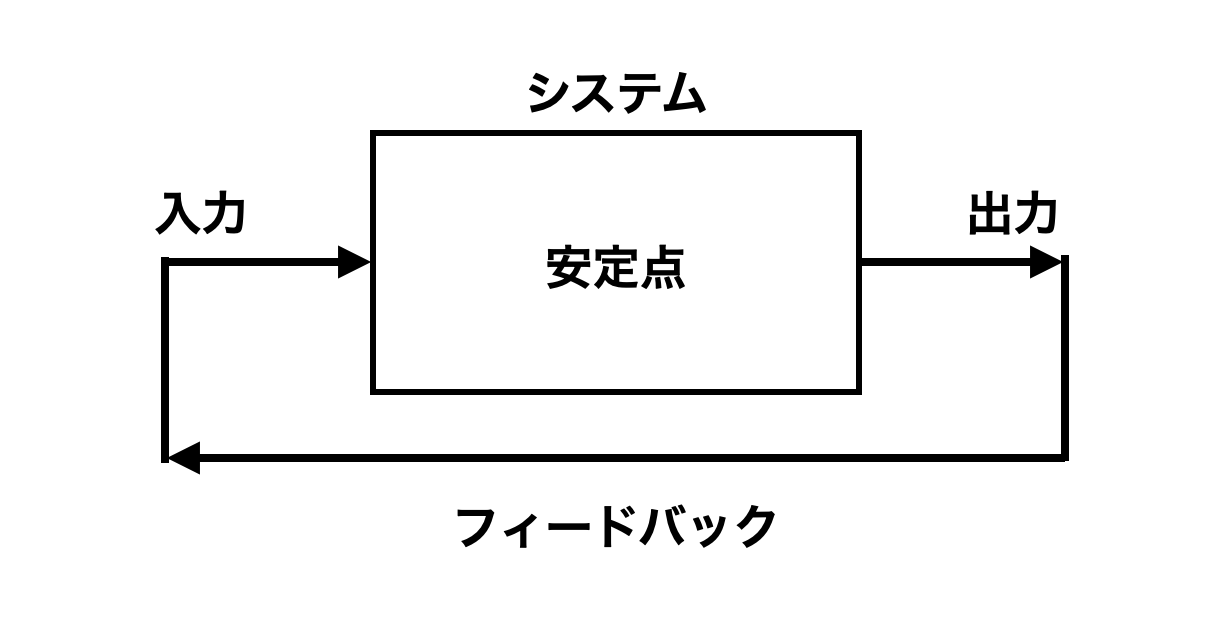
\includegraphics[keepaspectratio,width=0.7\linewidth]{../images/08_feedback.png}
	\caption{フィードバックを考えるサイバネティクス\index[termidx]{さいばねてぃくす@サイバネティクス}}
	\label{feedback_loop}
\end{figure}

システム論\index[termidx]{しすてむろん@システム論}的な発想は様々な分野に広がっていて，例えば心理学の分野では，ゲシュタルト心理学\index[termidx]{げしゅたるとしんりがく@ゲシュタルト心理学}にも似たような考え方が見られるんですね。プレグナンツの法則\footnote{プレグナンツの法則(Law of Pr\"{a}gnanz)は，ゲシュタルト心理学\index[termidx]{げしゅたるとしんりがく@ゲシュタルト心理学}における基本原則で，人間が視覚情報を可能な限り単純で秩序立った形として知覚する傾向を指します。この法則は視覚デザインや認知心理学\index[termidx]{にんちしんりがく@認知心理学}の研究において重要な役割を果たします。(Wikipediaより)}なんかがその例で，要素をある形で配置すると像が見えてくるという現象は，個々の要素の研究ではなく，要素間の関係性から生まれる全体性を扱っているわけです。これはベルタランフィ\index[nameidx]{べるたらんふぃ@ベルタランフィ}の一般システム論\index[termidx]{しすてむろん@システム論}と同時代の考え方で，同じような発想の基盤に立っているんですね。

さらに，システムの階層性という考え方も出てきます。システムって抽象的に聞こえますが，実は「何をシステムとみなすか」というのが重要なポイントなんです。例えば会社組織を考えてみると，会社全体を一つのシステムとして見ることができます。その中には生産部門，資材調達部門，営業部門，広告部門といった様々な部門があって，それぞれが協力し合って会社全体の安定的な利益を生み出しているシステムとして捉えることができるわけです。

会社を例にとると，まず会社全体を一つのシステムとして見ることができます。例えば，「これが売れそうだ」というインプットがあれば生産を増やす，逆に生産過剰で問題が起きれば減らすという具合に，全体としてバランスを取っているシステムとして捉えることができます。
一方で，その中の個々の部門もまたシステムとして見ることができます。例えば生産部門では，資材部から届いた材料に対して，どう生産を調整していくかという，より小さなシステムとして機能しているわけです。
つまり，大きなシステムの中に小さなシステムがあって，さらにその中にもより小さなサブシステムがある。例えば生産部門の中には，機械のライン調節部門や材料組立部門といった，様々なサブシステムが存在するわけです。
アーサー・ケストラー\index[nameidx]{けすとらー@ケストラー}は「機械の中の幽霊」という本\parencite{koestler1967ghost}の中で，ホロン\index[termidx]{ほろん@ホロン}という語でこの階層システムの特徴的な性質を指摘しています。中間的なシステムは，上位システムに対しては従属的な立場を取る一方で，下位システムに対しては統合的な役割を果たすというんですね。

この考え方は廣田君美によってグループダイナミックス\index[termidx]{ぐるーぷだいなみっくす@グループダイナミックス}の分野にも応用されました\parencite{HirotaKimiyoshi}。グループ全体，サブグループ，さらにその下のサブサブグループといった具合に，グループも階層的な構造を持っているという考え方です。
例えば，グループ人間関係を考えると，例えば僕は5人家族なんですが，5人家族という小さい系列という1つのシステムを持っています。その中にも親と子供は，子供は3人いますから，子供なりのコミュニケーションチャンネルがあるわけですね。親は親夫婦だけで会話するようなところもあるわけなので，小さいシステムの中には親システムと子システムが含まれている。何か意見を言うとか，子システムから親システムに進言するみたいな，システムレベル同士での話があったりします。もちろん，その中で，個々の人間，1人1人の人間としての存在もあります。親としては，この冬は温泉に行きたいと言ってるけれども，僕は個人的には行った先で漫画でも読んでゴロゴロしていたりなと思ってる，といったようにね。つまりメンバーもいろんなレベルでのシステムの関係性の中に入っているんです。動的平衡系\index[termidx]{どうてきへいこうけい@動的平衡系}の狙いは安定ですから，それぞれのレベルで安定を目的にしています。もちろん，小杉家という家族全員が幸せであるということが，幸せな状態で安定しているというのが良いわけですけれども，その安定の中にも，夫婦関係の安定，子供関係の安定，子供の中でも姉と弟の安定とか，それぞれのレベルでの安定があり得るわけです。

社会心理学\index[termidx]{しゃかいしんりがく@社会心理学}においてシステム論\index[termidx]{しすてむろん@システム論}が重要なのは，まさにこういった多層的な関係性を扱うからです。個人の対人関係レベル，集団レベル，マクロな社会レベルと，それぞれがネストされた構造を持ち，各レベルで安定を求めている。だから社会心理学\index[termidx]{しゃかいしんりがく@社会心理学}の核心は，これら複数のシステム間の安定性や相互作用を研究することにあるべきだということですね。
単に外的刺激に対する個人の反応を見るだけ，あるいはその刺激が社会的なものだからという理由だけで社会心理学\index[termidx]{しゃかいしんりがく@社会心理学}とするのではなく，こういったダイナミックなシステム間の相互作用を研究することが重要だという指摘は，非常に示唆的だと思いませんか。

ちなみに，第一世代システム\index[termidx]{だいいちせだいしすてむ@第一世代システム}の臨床心理学的な応用例が，家族システム論\index[termidx]{かぞくしすてむろん@家族システム論}というやつです。この考え方の特徴は，問題を個人に還元せず，家族全体をシステムとして捉えることです。
例えば，お姉ちゃんが高校に行かなくなっちゃった，不登校になったという場合，お姉ちゃん個人だけをケアしても根本的な解決にはならないと考える立場です。お姉ちゃんが問題だからお姉ちゃんをケアする，というのは直線的な因果関係ですよね。でもお姉ちゃんが元気になっても，また家族でしばらく暮らしているとだんだん不登校になっていく，というような繰り返しが起こったりします。なぜなら，その症状は家族関係全体の問題が個人に現れているからだ，というわけですね。このように，一つの原因が一つの結果になる，一つの問題を直せばあとは組み立てたら良い，という単順なものではなくて，一つが複数に影響する，複数が一つに影響するという多対多の因果関係を考えるために，システム論\index[termidx]{しすてむろん@システム論}的発想が必要なわけです。さらに，本人個人のシステムはもちろん，子どもたち同士のシステム，親子関係のシステム，そして家族全体のシステムといった，様々なレベルのシステムに注目して治療を進めていきます。この家族システム論\index[termidx]{かぞくしすてむろん@家族システム論}は，第一世代システム\index[termidx]{だいいちせだいしすてむ@第一世代システム}論と第三世代システム論\index[termidx]{しすてむろん@システム論}の影響を受けた治療アプローチを採用していて，システム論\index[termidx]{しすてむろん@システム論}的な見方が臨床心理学の実践でも有効に活用できることを示している良い例なんですね。

\subsection{第一世代システムの限界}

ということで，このシステム論\index[termidx]{しすてむろん@システム論}というのはどういうことを言わんとしているかということの方向性はお分かりいただけたかなと思うんですが，第一世代システム\index[termidx]{だいいちせだいしすてむ@第一世代システム}論の限界とか，次にどういったことが問題になってきたかということをちょっと指摘しておきたいと思います。まずは，この連立微分方程式\index[termidx]{れんりつびぶんほうていしき@連立微分方程式}で書いたことによる限界です。サイズ$n$の連立微分方程式\index[termidx]{れんりつびぶんほうていしき@連立微分方程式}という形で表現したことで，システムの要素数を固定してしまうという限界があったんですね。これはベルタランフィ\index[nameidx]{べるたらんふぃ@ベルタランフィ}自身は明示的に指摘していない問題点です。


最近生成AI\index[termidx]{せいせいえーあい@生成AI}ってすごいじゃないですか。生成AI\index[termidx]{せいせいえーあい@生成AI}，ChatGPTやClaudeといった生成AI\index[termidx]{せいせいえーあい@生成AI}は，まるで生きた知的な存在のように会話ができます。この講義録も彼ら？それら？の力を借りながらやるんですけど\footnote{録音したものを文字起こしするときに，OpenAI社のwhisperという機能を使っています。ここでは段落わけもない，文字列が生成されるんですが，口調を変えずに誤字脱字，誤変換を修正するようにOpenAIのAPIをPythonから呼び出して指示します。出来上がったものは私が自分で読んで加筆修正していますが，脚注を書かせたり書式ファイルを整えたり，索引のキーワードリストを作ったり，というところでClaudeの力を借りています。おかげで金曜日に講義が終わっても，よく実には清書した講義録ができるんです。}，すごくそれっぽい会話ができてます。まるで生きた人間かのように，知能があるかのように，生命かのようにやりとりができますね。プログラミングの相談をすれば，既存の効率的なプログラムの知識を組み合わせて答えを出してくれる。

でも，これらは結局のところ，すでに学習を終えた膨大だけれども固定的なデータセットに基づいて，それを組み合わせて出力しているわけです。一方で人間のシステムは，このインプットする要素の数$n$自体が状況に応じてダイナミックに変化していく。これが人間と現在のAIとの本質的な違いかもしれない，というわけですね。もちろん，これは個人的な考察であって，異なる見方もあり得るわけですが。

人間は新しい知識や言葉を作り出せるし，本を読んでボキャブラリーを増やしたり，情報を仕入れたりして，データセットをダイナミックに更新していけるわけです。「最近の子は本を読まない」とか「固定的な知識の中だけで議論する人が多い」という指摘は一旦置いておくとして，また人間がどれだけ頑張ってもチャットGPTの学習データセット量には及ばないかもしれませんが，原理的にそこが可変であるということが，人間の大事なポイントなんじゃないか，チャットGPTとの本質的な違いなんじゃないかと思うんです。
生命を持っているということは，このデータセットが変わり得るということなんじゃないかと。グループで考えてみても，例えば野球チームは9人という決まった人数でプレイしますが，本来の有機的なグループというのは，メンバーが出入りしても安定的な何かを維持できているもののはずなんです。
ベルタランフィ\index[nameidx]{べるたらんふぃ@ベルタランフィ}が連立微分方程式\index[termidx]{れんりつびぶんほうていしき@連立微分方程式}という形で表現した時に，システムの要素のサイズを固定せざるを得なかったということは，システム論\index[termidx]{しすてむろん@システム論}が考えるべき重要な限界の一つだったんじゃないかと思います。

連立微分方程式\index[termidx]{れんりつびぶんほうていしき@連立微分方程式}という表現方法を選んだこと自体も，大きな制約になっているといえるでしょう。なぜかというと，微分・積分というのはニュートン\index[nameidx]{にゅーとん@ニュートン}力学的な対称性を前提としているんですね。時間について微分できるということは，積分すれば元の状態に戻れるという対称性があることを意味している。でも，生命システムが扱う「時間の方向性」にそんな対称性があるのか，という根本的な問題があるわけです。この時間の非対称性という問題は，後の第二世代システム科学で，エントロピーの増大に関する議論として展開されていくことになります。
さらに，先ほどの要素数の固定という問題とも関連しますが，ベルタランフィ\index[nameidx]{べるたらんふぃ@ベルタランフィ}のシステム論\index[termidx]{しすてむろん@システム論}では生命の重要な特徴である増殖や修復，創出といった現象を扱えなかったという限界もあります。私たちの爪や髪の毛が切っても伸びてくるような再生能力や，生物が自分のコピーを作り出す能力といった，生命の本質的な特徴をこのシステムでは表現できなかったんですね。

システムを連立微分方程式\index[termidx]{れんりつびぶんほうていしき@連立微分方程式}で表現しようとしたことで，オープンで安定したシステムを数式的に記述することはできました。でも，これだけでは生命を十分に語れないという限界があったんです。

さらに，システム論\index[termidx]{しすてむろん@システム論}を扱う際の理論的な落とし穴もありました。「全体は要素の総和以上である」という考え方は，聞こえはいいんですが，これを強調しすぎると「だから全体なのだ」という全体還元主義\index[termidx]{ぜんたいげんげんしゅぎ@全体還元主義}に陥ってしまう危険性がある。しかも，その全体に向かおうとする方向性自体が，私たちが最初に否定すべきだった一直線の因果性や目的論を含んでしまいがちになる。そこは特に注意が必要なポイントだったわけですね。

こういった限界はあるんですけれども，ベルタランフィ\index[nameidx]{べるたらんふぃ@ベルタランフィ}が一般システム論\index[termidx]{しすてむろん@システム論}を立てたおかげで，一つのものの見方が成立したというのは評価すべきところではないかなと思います。皆さんはこの第一世代システム\index[termidx]{だいいちせだいしすてむ@第一世代システム}，動的平衡系\index[termidx]{どうてきへいこうけい@動的平衡系}というのをどのように捉えていただけましたでしょうか。自分なりにオープンなシステム，オープンで安定しているシステムというのを考えてみるというのが良いかなと思います。ちょっと考えてみてください。
\subsection{観察者問題}
ベルタランフィ\index[nameidx]{べるたらんふぃ@ベルタランフィ}が見落としていた重要な問題の一つに，観察者の位置づけという問題があります。システム論\index[termidx]{しすてむろん@システム論}は「ものの見方」だと言って，「これがインプットで，これがアウトプットだ」と定義し，サイズ$n$の関数で分析しようとしました。でも，そこには重要な問題が隠れているんですね。それは「このシステムをシステムだと見なした人は，いったいどこにいるのか」という問題です。
例えば空調システムの場合，エアコンを一つのシステムとして，外気をインプットして設定温度に合わせてアウトプットすると説明する時，「これがシステムです」と言っている人は明らかにシステムの外側にいるわけです。そして外からシステムの安定点として「23度です」と設定している。

でも，ここで考えてみてほしいのは生き物の場合です。皆さんは生きていますよね。でも皆さんの「安定」は誰が決めているんでしょう？私があなたの体温はこれくらいですよ，と決めたわけではありませんよね。あなたの幸せはこの程度ですよ，なんて決められるわけがない。

自分というのが，このボディの物理的なものだけだと皆さんはお考えでしょうか？もしそうだとしたら，自分の境界線ははっきりしていますが，自分，自己，生命というのは，少なくとも物理的なものだけじゃないですよね。この辺はうまく言語化しにくいんですが，いつしかここに小さい妖精さんがいると考えて，みたいな話をしました。あそこで論じたように，自分の社会的実在\index[termidx]{しゃかいてきじつざい@社会的実在}性を考えるのであれば物理的な境界は必要ありません。

システムは社会的に実在していればいいのであって，物理的な実体が必要ではない。グループというのは目に見えない全体なので，見える必要はない。この教室の中に入った人がグループです，という操作的定義でも，良いと言えば良いかもしれませんが，そんなはずないじゃないですか。物理的なグループの境界というのは，物理的に決められるものではないはずです。ということは同時に，人間の私の境界というのも，別にこの物理的な基盤を持っていることを否定はしませんが，そんな形がなかったとしても，その人個人のシステムというのは実在していればいいわけなので，物理的境界に固定されているわけではないわけです。

何が言いたいかというと，生命とは，生きているとは，グループであるとは，自分があるというのは，外から観察されているわけじゃないんですよ。自分で決めているんです。自分の安定点というのも自分で作っているんです。この自己を持っているというのが，この生命の特別な性質なので，この自己をどう扱いますかというのが，第二，第三世代のシステムに関わってきます。そのつもりで，次回以降のお話を聞いていただければと思います。

\subsection{社会心理学における動的平衡系}
最後に，申し訳程度に，社会心理学\index[termidx]{しゃかいしんりがく@社会心理学}における動的平衡系\index[termidx]{どうてきへいこうけい@動的平衡系}という話題を用意しておきましょう。

家族システムの話はさきほども言った通りです。臨床系の家族システム論\index[termidx]{かぞくしすてむろん@家族システム論}というものの中では，このベルタランフィ\index[nameidx]{べるたらんふぃ@ベルタランフィ}システムの観点で，因果的な直線的な要素，還元主義的な治療，介入をしないでおこうというような方針として運用されています。治療的な話がなかったとしても，社会心理学\index[termidx]{しゃかいしんりがく@社会心理学}におけるグループや，家族の考え方もあるでしょうから，社会心理学\index[termidx]{しゃかいしんりがく@社会心理学}における動的平衡系\index[termidx]{どうてきへいこうけい@動的平衡系}という意味で，家族やグループというのを考えることもできるでしょう。

それともう一つは，いつしか社会心理学\index[termidx]{しゃかいしんりがく@社会心理学}の歴史の中でお話ししましたが，ハイダーやニューカム\index[nameidx]{にゅーかむ@ニューカム}，オズグットとタネンバウム\index[nameidx]{たねんばうむ@タネンバウム}，フェスティンガー\index[nameidx]{ふぇすてぃんがー@フェスティンガー}などが考えた認知均衡理論というのがありましたね。バランス理論です。インバランスしていたらバランスした状態に戻そうとしますよ。バランス理論というのも，社会心理学\index[termidx]{しゃかいしんりがく@社会心理学}における動的平衡系\index[termidx]{どうてきへいこうけい@動的平衡系}の観点を持っているものですね。いろんな認知的な要素があるんだけど，それが安定的な全体性になるように，情報のインプット・アウトプットをしながら，安定的な心の状態を保とうとする考え方なわけです。なので，バランス理論というのも，第一世代システム\index[termidx]{だいいちせだいしすてむ@第一世代システム}的な発想を持った考え方なんじゃないかなと思います。

最後に多変量解析ですね。社会心理学\index[termidx]{しゃかいしんりがく@社会心理学}の具体的な研究方法として，社会調査つまりアンケート調査，調査票によるデータを対応にとって，それを分析して，何かモデルを立てるというような研究が主流です。このことに関する批判は，また後半の方でやっていこうかなと思うんですけれども，多変量解析，社会調査による分析方法というのは，アンケート調査票というデータに含まれる安定的な構造を取り出そうという考え方です。その取り出した構造によって，このアンケート調査の空間の中には，「こういう要素，こういう要素，そしてこういう要素がありましたよ」というような言い方をします。因子分析によって，因子を抽出するなんて言ったりします。しかし，「あの因子がある」というのは，具体的な厳密な話をすると，一人一人の心の中にあるわけではありません。社会だとか言語空間の中に，因子という安定的な構造が存在しています。そこに調査協力者，あるいは被験者，といった人を作用させる。人に項目のセットを与えると，因子によって変換されますよ，ということなんです。

線形代数でいうところの写像だとか，「行列による座標変換の話」といった知識がないと，この話も中途半端になってしまうんですが。言語空間における安定的な要素間関係を記述しましょう，というのが大変重要なのです。主成分分析とか因子分析というのは，言語空間における要素間関係を記述するための方法です。なので，こういった調査方法なんかも基本的には動的平衡系\index[termidx]{どうてきへいこうけい@動的平衡系}です。言語空間というのはきっとこういう因子で安定しているでしょう。そうすると，人が社会問題に対して意識を持ったら，「こういう3つの要素に分かれます」といったような形でモデル化されているのが非常に理解しやすいです。そういったものとして，社会心理学\index[termidx]{しゃかいしんりがく@社会心理学}の中でも動的平衡系\index[termidx]{どうてきへいこうけい@動的平衡系}の考え方が生きている，ということについて，最後にちょっと触れておきたかったんです。



はい，今日は「システム論\index[termidx]{しすてむろん@システム論}の導入」ということで，第一世代システム\index[termidx]{だいいちせだいしすてむ@第一世代システム}をしっかりと学んだつもりです。次回は第二，第三世代のシステムについてお話を進めていきたいと思います。その時のテーマは先ほども言いましたが，「自己の境界をどうするか」というようなことと，それに含めて「観察者の問題」なんかが入ってきますので，どうぞお楽しみに。

はい，それでは今日の話はここまでにしておきましょう。お疲れ様でした。

\printbibliography[title=引用文献]

\end{document}

